%--------------------------------------------------------------
\section{نقاط تعادلِ لاگرانژ}\label{sec:lag-points}

نقطه‌ی تعادل مکانی است که در چارچوبِ چرخان، جرمِ سوم بی‌حرکت می‌ماند. این شرط با صفر شدن مؤلفه‌های سرعت و شتاب حاصل می‌شود؛ ازاین‌رو در معادلاتِ حرکتِ بخش \ref{sec:crtbp} قرار می‌دهیم $\dot x=\dot y=\dot z=\ddot x=\ddot y=\ddot z=0$. در نتیجه دستگاهِ جبریِ زیر برای مختصاتِ نقطه‌ی تعادل به‌دست می‌آید:
\begin{align}
	0 &= x-\frac{1-\mu}{r_{1}^{3}}(x+\mu)-\frac{\mu}{r_{2}^{3}}\bigl(x-1+\mu\bigr),\\
	0 &= y\Bigl[1-\frac{1-\mu}{r_{1}^{3}}-\frac{\mu}{r_{2}^{3}}\Bigr],\\
	0 &= -\frac{1-\mu}{r_{1}^{3}}\,z-\frac{\mu}{r_{2}^{3}}\,z.
\end{align}
معادله‌ی سوم نشان می‌دهد در حالتِ عمومی باید $z=0$ باشد؛ بنابراین، نقاطِ تعادل همگی در صفحه‌ی مدار قرار می‌گیرند.

\subsubsection{دسته‌بندی کلی}
\begin{enumerate}
	\item {
		نقاطِ هم‌خط\LTRfootnote{Collinear}:
	} سه نقطه‌ی $L_{1}$، $L_{2}$ و $L_{3}$ روی خطِ واصلِ دو جرم قرار دارند و لذا $y=0$ است.
	\item {
		نقاطِ سه‌گوش\LTRfootnote{Triangular}:
		.} دو نقطه‌ی $L_{4}$ و $L_{5}$ رأس‌های مثلثِ متساوی‌الاضلاع با دو جرمِ اصلی را تشکیل می‌دهند و در آن‌ها $y\ne0$.
\end{enumerate}

\begin{figure}[H]
	\centering
	\begin{tikzpicture}
		% Define radius of the orbit
		\def\orbitRadius{4cm}
		
		% Draw the orbit circle with arrows
		\draw[-{Stealth[length=3mm]}, thick] (12:\orbitRadius) arc (12:170:\orbitRadius);
		\draw[-{Stealth[length=3mm]}, thick] (180:\orbitRadius) arc (180:355:\orbitRadius);
		
		% Position for Earth (center)
		\node[inner sep=0pt] (Earth) at (0,0) {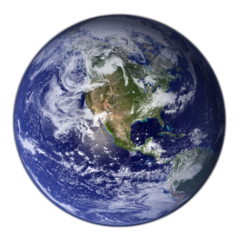
\includegraphics[width=1.8cm]{../Figure/TBP/Earth.png}};
		\node[text=black] at (0,-1.3) {زمین};
		
		% Position for Moon (on the right side of the orbit)
		\node[inner sep=0pt] (Moon) at (0.95*\orbitRadius,0) {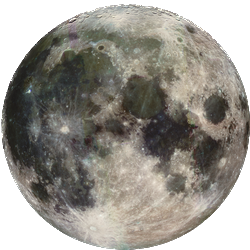
\includegraphics[width=0.6cm]{../Figure/TBP/Moon.png}};
		\node[text=black] at (\orbitRadius,0.6) {ماه};
		
		% Lagrangian points
		\coordinate (L1) at (0.8*\orbitRadius,0);
		\coordinate (L2) at (1.2*\orbitRadius,0);
		\coordinate (L3) at (-1*\orbitRadius,0);
		\coordinate (L4) at (60:\orbitRadius);
		\coordinate (L5) at (300:\orbitRadius);
		
		% Draw Lagrangian points as red circles
		\foreach \point in {L1,L2,L3,L4,L5} {
			\fill[red] (\point) circle (0.1cm);
		}
		
		% Connect Lagrangian points with dashed lines
		\draw[dashed, blue, thick] (Earth) -- (L1);
		\draw[dashed, blue, thick] (Moon) -- (L1);
		\draw[dashed, blue, thick] (Moon) -- (L2);
		\draw[dashed, blue, thick] (Earth) -- (L3);
		\draw[dashed, blue, thick] (Earth) -- (L4);
		\draw[dashed, blue, thick] (Moon) -- (L4);
		\draw[dashed, blue, thick] (Earth) -- (L5);
		\draw[dashed, blue, thick] (Moon) -- (L5);
		
		% Labels for the Lagrangian points
		\node at ($(L1) + (0,0.5)$) {$L_1$};
		\node at ($(L2) + (0,0.5)$) {$L_2$};
		\node at ($(L3) + (0,0.5)$) {$L_3$};
		\node at ($(L4) + (0.5,0.3)$) {$L_4$};
		\node at ($(L5) + (0.5,-0.3)$) {$L_5$};
	\end{tikzpicture}
	\caption{نقاطِ لاگرانژ در سامانه‌ی زمین–ماه}
\end{figure}

%--------------------------------------------------------------
\subsubsection{نقاطِ هم‌خط \texorpdfstring{$(L_{1},L_{2},L_{3})$}{(L1,L2,L3)}}\label{subsec:collinear}

با اعمال $y=0$، تنها معادله‌ی زیر باقی می‌ماند:
\begin{equation}\label{eq:collinear_eq}
	x-\frac{1-\mu}{|x+\mu|^{3}}(x+\mu)-\frac{\mu}{|x-1+\mu|^{3}}\bigl(x-1+\mu\bigr)=0.
\end{equation}
این معادله در سه ناحیه‌ی مجزا—بین دو جرم، بیرونِ جرمِ کوچک و بیرونِ جرمِ بزرگ—دارای یک ریشه است که به‌ترتیب نقاطِ $L_{1}$، $L_{2}$ و $L_{3}$ را تعیین می‌کند.

برای $\mu\ll1$ (همچون سامانه‌ی خورشید–زمین یا زمین–ماه) می‌توان تقریب‌های شناخته‌شده را نوشت:
\begin{align*}
	x_{L_{1}} &\simeq (1-\mu)-\bigl(\tfrac{\mu}{3}\bigr)^{1/3},\\
	x_{L_{2}} &\simeq (1-\mu)+\bigl(\tfrac{\mu}{3}\bigr)^{1/3},\\
	x_{L_{3}} &\simeq -1-\tfrac{5}{12}\,\mu; \qquad y_{L_{i}}=0.
\end{align*}
در عمل، ریشه‌ی دقیقِ معادله‌ی \eqref{eq:collinear_eq} با یک روشِ عددی (نیوتن–رافسون) محاسبه می‌شود.

%--------------------------------------------------------------
\subsubsection{نقاطِ سه‌گوش \texorpdfstring{$(L_{4},L_{5})$}{(L4,L5)}}\label{subsec:triangular}

در این نقاط $r_{1}=r_{2}=1$ و شرطِ
\(1-(1-\mu)/r_{1}^{3}-\mu/r_{2}^{3}=0\)\, به‌طور طبیعی برقرار است. مختصات به  عبارت‌اند از
\begin{equation}
	x_{L_{4}}=x_{L_{5}}=\tfrac12-\mu,\qquad
	y_{L_{4}}=+\tfrac{\sqrt3}{2},\qquad
	y_{L_{5}}=-\tfrac{\sqrt3}{2}.
\end{equation}
پایداری این نقاط مستلزم نسبتِ جرمِ کافی است؛ شرطِ کلاسیک~$m_{1}/m_{2}>24.96$ (یا معادل آن $\mu<\mu_{\mathrm R}\approx0.03852$) در سامانه‌های خورشید–سیاره یا زمین–ماه برقرار است و سببِ وجودِ خانواده‌ی سیارک‌های تروجان حول $L_{4}$ و $L_{5}$ می‌شود. در مقابل، نقاطِ هم‌خط ناپایدارند و معمولاً مأموریت‌های فضایی روی مدارهای هاله‌ای یا لیساژور در پیرامونِ آن‌ها قرار می‌گیرند.

%--------------------------------------------------------------
% \subsubsection{مثال: سامانه‌ی زمین–ماه}\label{subsec:earth-moon}

برای سامانه‌ی زمین–ماه، $\mu\simeq0.01215$ است. جدولِ زیر مختصاتِ بی‌بُعدِ هر پنج نقطه را نشان می‌دهد (واحدِ طول: فاصله‌ی زمین–ماه). موقعیتِ زمین در $(-\mu,0)$ و ماه در $(1-\mu,0)$ است.

\begin{table}[H]
	\centering
	\caption{مقادیر عددی نقاط لاگرانژ برای مسئله‌ی سه‌جسمیِ محدودِ سیستمِ زمین–ماه}
	\begin{tabular}{|c|c|c|}
		\hline
		\text{نقطه‌ی لاگرانژ} & \(x\) \, (\text{بی‌بعد}) & \(y\) \, (\text{بی‌بعد}) \\
		\hline
		$L_1$ & $+0.83692$ & $0$ \\
		$L_2$ & $+1.15568$ & $0$ \\
		$L_3$ & $-1.00506$ & $0$ \\
		$L_4$ &$ +0.48785$ & $+0.86603$ \\
		$L_5$ & $+0.48785$ & $-0.86603$ \\
		\hline  
	\end{tabular}
	\label{tab:lag-earth-moon}
\end{table}

این نتایج نشان می‌دهد که $L_{1}$ در حدودِ $0.84$ فاصله‌ی زمین–ماه از زمین قرار دارد (فاصله‌ی آن تا ماه در حدود $0.16$ واحد طول است) و $L_{2}$ بیرونِ مدارِ ماه است. نقطه‌ی $L_{3}$ تقریباً یک واحدِ طول در سوی مقابلِ ماه نسبت به زمین قرار دارد. دو نقطه‌ی $L_{4}$ و $L_{5}$ در مختصات $(0.488,\pm0.866)$ قرار گرفته و با زمین و ماه مثلثِ متساوی‌الاضلاع می‌سازند.
%		$L_5$ & $+0.48785$ & $-0.86603$ \\
%		\hline  
%	\end{tabular}
%\end{table}

این نتایج نشان می‌دهد که $L_{1}$ در حدودِ $0.84$ فاصله‌ی زمین–ماه از زمین قرار دارد (فاصله‌ی آن تا ماه در حدود $0.16$ واحد طول است) و $L_{2}$ بیرونِ مدارِ ماه است. نقطه‌ی $L_{3}$ تقریباً یک واحدِ طول در سوی مقابلِ ماه نسبت به زمین قرار دارد. دو نقطه‌ی $L_{4}$ و $L_{5}$ در مختصات $(0.488,\pm0.866)$ قرار گرفته و با زمین و ماه مثلثِ متساوی‌الاضلاع می‌سازند.
